\documentclass[tikz,border=10pt]{standalone}
\usetikzlibrary{arrows.meta}

\begin{document}

{\sffamily

\tikzset{every loop/.style={min distance=10mm}} % removes arrow head from all loops.

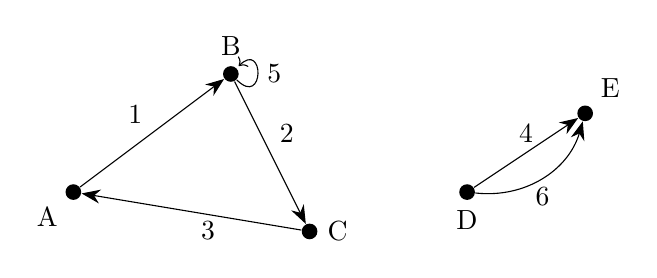
\begin{tikzpicture}[
	    arrow style/.style={-{Stealth[scale=1.4]}},
]

% Triangle component
\node (A) at (1,2) [circle, fill=black, inner sep=2pt, label=below left:A] {};
\node (B) at (3,3.5) [circle, fill=black, inner sep=2pt, label=above:B] {};
\node (C) at (4,1.5) [circle, fill=black, inner sep=2pt, label=right:C] {};

\draw[arrow style] (A) -- node[above left] {1} (B);
\draw[arrow style] (B) -- node[above right] {2} (C);
\draw[arrow style] (C) -- node[below right] {3} (A);

% Circular loop at B (edge 5)
\draw[arrow style] (B) edge[in=45, out=-45, loop] node[right] {5} ();

% Two-node component
\node (D) at (6,2) [circle, fill=black, inner sep=2pt, label=below:D] {};
\node (E) at (7.5,3) [circle, fill=black, inner sep=2pt, label=above right:E] {};

\draw[arrow style] (D) -- node[above] {4} (E);
\draw[arrow style] (D) to[bend right=40] node[below] {6} (E);

\end{tikzpicture}

}

\end{document}